\documentclass[]{article}
\usepackage{lmodern}
\usepackage{amssymb,amsmath}
\usepackage{ifxetex,ifluatex}
\usepackage{fixltx2e} % provides \textsubscript
\ifnum 0\ifxetex 1\fi\ifluatex 1\fi=0 % if pdftex
  \usepackage[T1]{fontenc}
  \usepackage[utf8]{inputenc}
\else % if luatex or xelatex
  \ifxetex
    \usepackage{mathspec}
  \else
    \usepackage{fontspec}
  \fi
  \defaultfontfeatures{Ligatures=TeX,Scale=MatchLowercase}
\fi
% use upquote if available, for straight quotes in verbatim environments
\IfFileExists{upquote.sty}{\usepackage{upquote}}{}
% use microtype if available
\IfFileExists{microtype.sty}{%
\usepackage{microtype}
\UseMicrotypeSet[protrusion]{basicmath} % disable protrusion for tt fonts
}{}
\usepackage[margin=1in]{geometry}
\usepackage{hyperref}
\hypersetup{unicode=true,
            pdftitle={Measuring the impact of new vaccines using mortality and administrative hospitalization data},
            pdfborder={0 0 0},
            breaklinks=true}
\urlstyle{same}  % don't use monospace font for urls
\usepackage{graphicx,grffile}
\makeatletter
\def\maxwidth{\ifdim\Gin@nat@width>\linewidth\linewidth\else\Gin@nat@width\fi}
\def\maxheight{\ifdim\Gin@nat@height>\textheight\textheight\else\Gin@nat@height\fi}
\makeatother
% Scale images if necessary, so that they will not overflow the page
% margins by default, and it is still possible to overwrite the defaults
% using explicit options in \includegraphics[width, height, ...]{}
\setkeys{Gin}{width=\maxwidth,height=\maxheight,keepaspectratio}
\IfFileExists{parskip.sty}{%
\usepackage{parskip}
}{% else
\setlength{\parindent}{0pt}
\setlength{\parskip}{6pt plus 2pt minus 1pt}
}
\setlength{\emergencystretch}{3em}  % prevent overfull lines
\providecommand{\tightlist}{%
  \setlength{\itemsep}{0pt}\setlength{\parskip}{0pt}}
\setcounter{secnumdepth}{0}
% Redefines (sub)paragraphs to behave more like sections
\ifx\paragraph\undefined\else
\let\oldparagraph\paragraph
\renewcommand{\paragraph}[1]{\oldparagraph{#1}\mbox{}}
\fi
\ifx\subparagraph\undefined\else
\let\oldsubparagraph\subparagraph
\renewcommand{\subparagraph}[1]{\oldsubparagraph{#1}\mbox{}}
\fi

%%% Use protect on footnotes to avoid problems with footnotes in titles
\let\rmarkdownfootnote\footnote%
\def\footnote{\protect\rmarkdownfootnote}

%%% Change title format to be more compact
\usepackage{titling}

% Create subtitle command for use in maketitle
\providecommand{\subtitle}[1]{
  \posttitle{
    \begin{center}\large#1\end{center}
    }
}

\setlength{\droptitle}{-2em}

  \title{Measuring the impact of new vaccines using mortality and administrative
hospitalization data}
    \pretitle{\vspace{\droptitle}\centering\huge}
  \posttitle{\par}
  \subtitle{Pneumococcal conjugate vaccine as a case study}
  \author{}
    \preauthor{}\postauthor{}
    \date{}
    \predate{}\postdate{}
  

\begin{document}
\maketitle

{
\setcounter{tocdepth}{3}
\tableofcontents
}
\begin{center}
\includegraphics[width=0.328\linewidth]{WHO_logo} \end{center}

\subsection{Introduction (Cris)}\label{introduction-cris}

Once vaccines or other public health interventions are deployed, it is
often desirable to measure their impact on health. This information is
often critical for policy-makers who prioritize funding and
implementation of different programs. However, conducting robust and
credible evaluations of the public health impact of interventions is
challenging. Real-world data are complex, and decisions about how to
clean, format, analyze, and interpret the data can influence the
conclusions about the impact of the intervention.

In this manual, we discuss issues in performing impact analyses using
routinely-collected administrative data sources. As a specific case
study, we discuss challenges in evaluating the impact of the
introduction of pneumococcal conjugate vaccines among children on rates
of hospitalization and death due to pneumonia.

\subsection{\texorpdfstring{What is vaccine
`impact'?}{What is vaccine impact?}}\label{what-is-vaccine-impact}

Many vaccines influence disease rates in 2 ways. Direct effects reduce
the risk for an individual to become ill and directly results from the
immune response from the vaccine. Indirect effects are the benefit that
an individual receives as a result of decreased transmission of the
pathogen. Both vaccinated and unvaccinated individuals benefit from this
indirect protection. When we refer to \emph{vaccine impact} we are
referring to the overall change in disease rates in the population that
results from the combination of direct and indirect effects.

\subsection{Mortality data from Vital Statistics
(Cris)}\label{mortality-data-from-vital-statistics-cris}

\subsection{Hospitalization data from administrative sources
(Cris)}\label{hospitalization-data-from-administrative-sources-cris}

\subsection{Study design (DAN)}\label{study-design-dan}

\subsubsection{Overview}\label{overview}

Observational studies present a number of analytical challenges. The
introduction of vaccines is often occurring concurrently with other
oublic health and social interventions that can influence disease rates.
Other relevant changes include changes in social welfare systems,
changes in the capacity of the healthcare system, changes in the
efficincy of registering hospitalizations and deaths, and other
pharmacological interventions that could influence susceptibility (e.g.,
increasing use of anti-retroviral therapy in sub-Saharan Africa).
Because vaccines are introduced at the same time as these other changes,
it can be challenging to attribute specific changes to the introduction
of a vaccine. The methods that we will discuss here attempt to address
this issue using different approaches and different assumptions. It is
important to be aware of the assumptions and limitations of the
different approaches.

\subsubsection{Possible study designs for impact
assessment}\label{possible-study-designs-for-impact-assessment}

The analysis goal is to disentangle changes in disease rates that are
caused by the introduction of a vaccine program with changes that are
due to these other factors. There are several approaches that could be
taken. First, in a \emph{pre-licensure} study, vaccine impact could be
evaluated using a cluster-randomized study design, where disease rates
are compared between spatial clusters that have been randomized to
receive that vaccine or not. Assuming that there is not transmission
between clusters, that the assignment of clusters was random and
succesful (i.e., that the vaccinated and unvaccinated clusters are
comparable), this provides an unbiased estimate of the total effect of
the vaccine.

In a \emph{post-licensure setting}, the cluster-randomized design can be
approximated by using a `step-wedge' study design. This design can be
implemented in settings where the vaccine has not yet be introduced and
where it might not be feasible to introduce to the entire population at
the same time. With this design, geographic areas are randomized to
receive the vaccine earlier or later. All geographic units eventually
receive the vaccine. With this phased rollout, the geographic units that
introduce the vaccine later serve as controls for the geographics units
that introduce the vaccine earlier. Because the control group is
changing over time and the comparisons between the vaccinated and
unvaccinated groups is taking place over some time period, estimates of
vaccine impact could be cofounded by underlying temporal trends.
Therefore, it is important to appropriately adjust for time-varying
rates of disease when analyzing these studies.

In most settings, such controlled roll-outs of vaccine are not possible.
Therefore, the most common study designs are purely observational, in
which changes in disease rates are evaluated over time or between
regions. Extreme caution needs to be used when performing and
interpreting these studies to ensure that factors unrelated to
vaccination are appropriately adjusted in the analysis. This guide will
focus on the analysis situation where there is a single time series of
interest from a country or region and the goal is to detect changes in
incidence following vaccine introduction from this time series. When
time series from multiple subnational regions are available, additional
types of analyses are possible, including performing spatiotemporal
analyses in which the declines in regions with higher or lower coverage
are compared.

\subsubsection{Counterfactuals: What would have happened without a
vaccine?}\label{counterfactuals-what-would-have-happened-without-a-vaccine}

With any analysis of vaccine impact, the goal is to compare the observed
disease rates in the post-vaccine period with an estimate of what would
have happened if the vaccine had not been introduced. This value is
called the \textbf{counterfactual}. There are many ways to estimate
counterfactuals from very simple approaches (as is done in pre/post
comparison of incidence) to more complex approaches that adjust for
trends and dynamics of the disease. In each of the followinng sections,
we will discuss different methods to obtain this quantity.

\subsection{Types of analyses}\label{types-of-analyses}

In this context, a `time series' is defined as a variable in which the
number of cases is tallied in each unit of time
(week/month/quarter/year). The goal for the analysis is to detect
changes in the average number of cases or incidence. In this example, we
have the number of hospitalization coded as having a diagnosis for
pneumonia (ICD10 codes J12-J18) in Brazil in infants

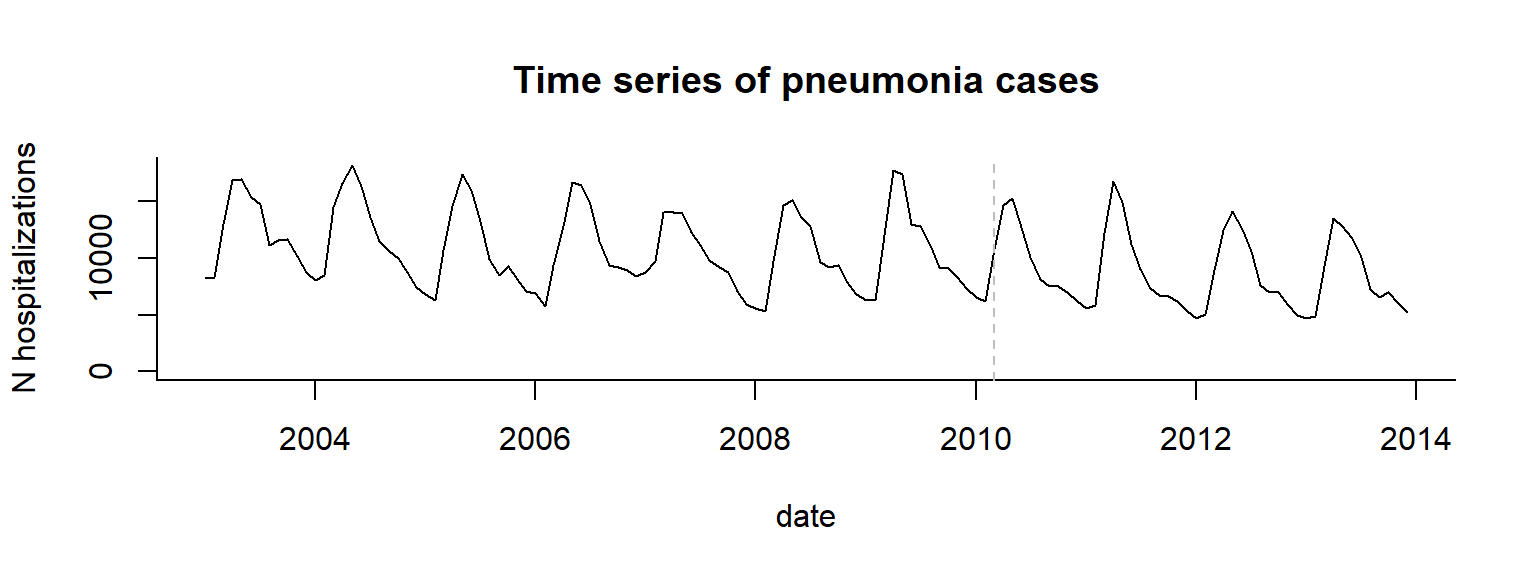
\includegraphics{WHO-guidance-on-use-of-administrative-data_files/figure-latex/unnamed-chunk-1-1.pdf}

\subsubsection{Key considerations for
analyses}\label{key-considerations-for-analyses}

What denominator, if any? How are denominators incorporated (as offset)
-Rollout period

\subsubsection{Pre-Post comparison}\label{pre-post-comparison}

The simplest possible analysis approach is to compare the average number
of cases or incidence in the post-vaccine period with that in the
pre-vaccine period (a `pre/post comparison' study). This method is easy
to implement and easy to understand. The analyst needs to define the
pre-vaccine period and the post-vaccine period. Typically, the first
year or two after vaccine introducion are excluded from the analysis
because vaccine coverage has not yet reached full coverage levels. The
decision about where to set the pre- and post-vaccine periods should be
made \emph{a priori} and should not be influenced by observed
aberrations in the data (unless these are due to a known data quality
issue); otherwise the estimation of the variability in disease rates
will not be accurate.

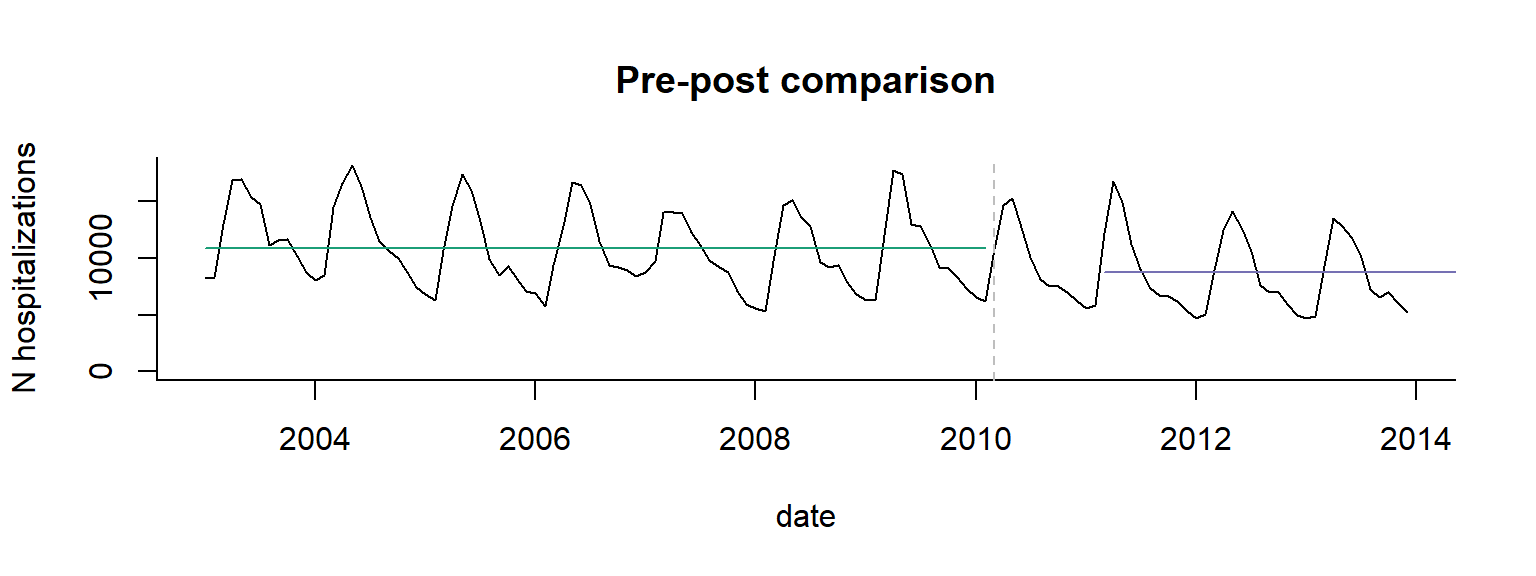
\includegraphics{WHO-guidance-on-use-of-administrative-data_files/figure-latex/unnamed-chunk-2-1.pdf}

\textbf{Counterfactual} In this study design, it is assumed that if the
vaccine had not been introduced, the incidence rate after vaccine
introduction would be the same as the incidence of disease before
vaccine introduction. Therefore the counterfactual is simply the average
incidence in the pre-vaccine period, and the comparison is with
incidence in the post vaccine period. In the plot below, the
\(\color{#d95f02}{\text{counterfactual}}\) is shown with a dotted line.
Comparing the \(\color{#d95f02}{\text{counterfactual}}\) with the
\(\color{#7570b3}{\text{observed mean for the post-period}}\) gives an
estimate of the vaccine effect.

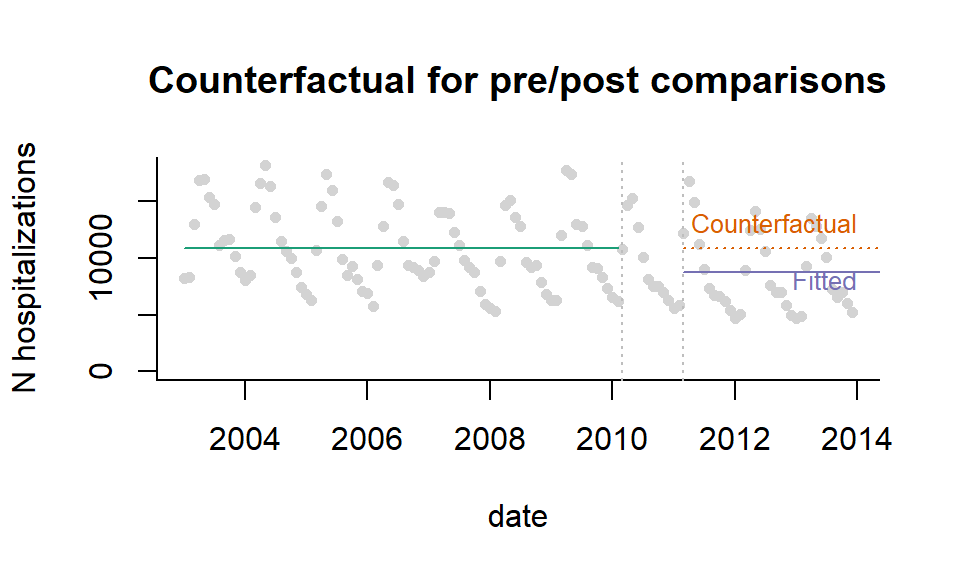
\includegraphics{WHO-guidance-on-use-of-administrative-data_files/figure-latex/unnamed-chunk-3-1.pdf}

\textbf{Calculation of vaccine impact} The most common statistic
reported from a pre/post comparison study is a Rate Ratio, which is
simply calculated as (Average Incidence Post-Vaccination)/(Average
Incidence Pre-Vaccination). Values \textless{}1 are considered evidence
that the disease rates have declined. It is also possible to calculate a
rate difference to obtain the number of cases prevented.

\textbf{Assumptions} This analysis assumes that the only change in
disease rates that is occurring over time is due to the vaccine. This is
rarely a realistic assumption. \textbf{Therefore, this is a weak study
design, and the results should be interpreted with caution.}

\textbf{Extensions} It is sometimes desirable to adjust for seasonality
in the analysis. This is particularly important when partial years are
included in the pre and/or post period, and the pre- or post-periods are
imbalanced in terms of which parts of the year are included in the
analyses. This is accomplished in a regression model by adjusting for
seasonality using dummy variables for month or harmonic variables. More
details can be found in the hands-on exercises.

In this example, the \(\color{#d95f02}{\text{counterfactual}}\) is
seasonally adjusted, so the counterfactual for January is equal to the
mean number of cases in January in the pre-vaccine period, and likewise
for all of the months.

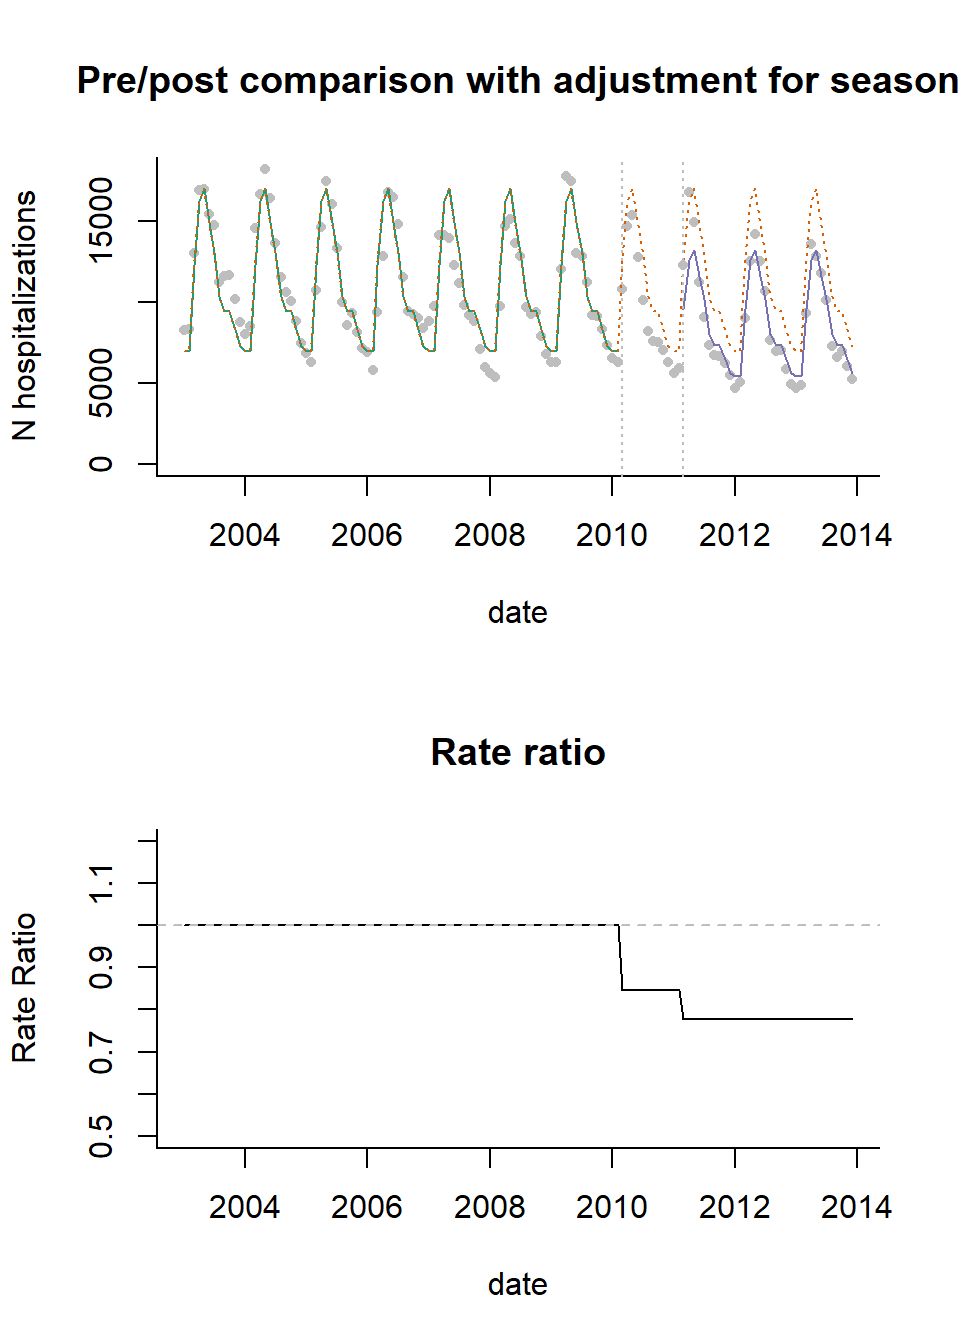
\includegraphics{WHO-guidance-on-use-of-administrative-data_files/figure-latex/unnamed-chunk-4-1.pdf}

\subsubsection{Interrupted time series analysis
(ITS)}\label{interrupted-time-series-analysis-its}

In many instances, there is an underlying trend in the time series that
is unrelated to vaccination. Such a trend can be caused by a number of
factors, including changes in healthcare access, changes in
susceptibility of the population, and changes in the sensitivity of
surveillance. Such trends can bias the estimates of vaccine impact if
they are not properly controlled. The simplest approach to adjust for
trends is to fit a straight line through the data and then test whether
the slope of the line or the level of the line changes after vaccine
introduction. This can be accomplished by fitting a Poisson or negative
binomial regression model. A number of quantities can be estimated sing
these models, including the change in the slope of the trend line or in
the average number of cases. However, it is often most useful to use the
model to calculate the decline in incidence (rate ratio or rate
difference) compared to what would be expected if the trend/level had
remained constant.

There are a number of ways to code these models, but they typically
include an index for time to capture the slope during the pre-vaccine
period as well as terms that allow the slope or intercept to change in
the post-vaccine period. The structure of the ITS model depends on how
quickly you expect the vaccine effect to take hold. An excellent review
of this topic is provided by Bernal, Cummins and Gasparrini (Intl Journ
of Epidem., 2017 (46)1: 348-355).

\paragraph{Disjointed ITS}\label{disjointed-its}

In a disjointed ITS analysis, dummy variables (encoded 0 before vaccine
introduction and 1 after vaccine introduction) are included to allow the
level to change, and an interaction term between the dummy variable and
the index for time allows the slope to change after vaccine
introduction. In this model, the line segments fitted through the data
do not connect. In practice, this can also lead to strange and
implausible shifts in the fitted values as shown in the plots of the
rate ratio below.

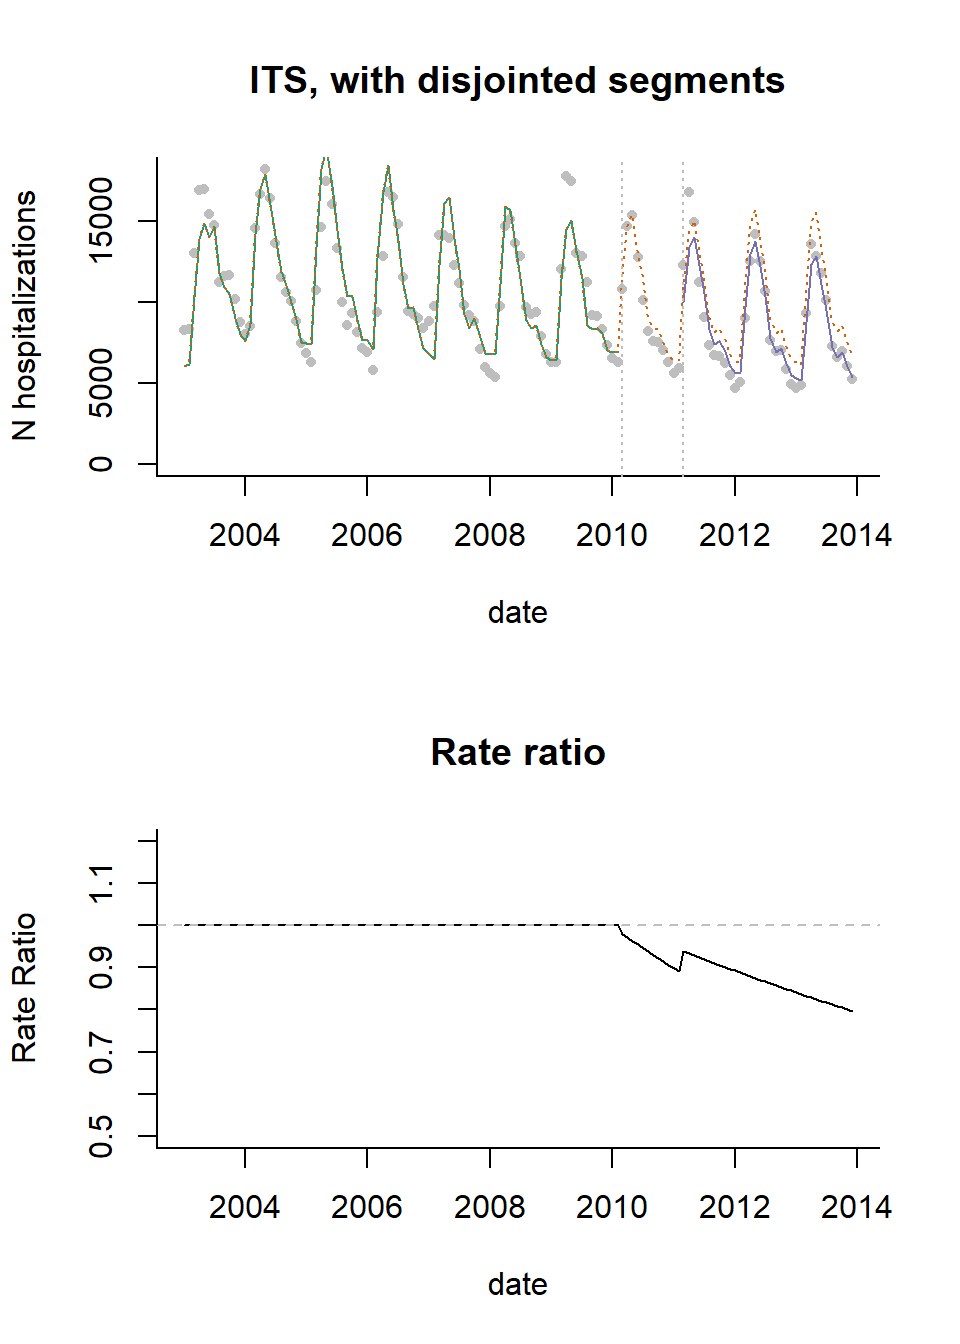
\includegraphics{WHO-guidance-on-use-of-administrative-data_files/figure-latex/unnamed-chunk-5-1.pdf}

\paragraph{ITS with connected
segments}\label{its-with-connected-segments}

A better alternative is to use a linear spline, which forces the fitted
line segments to connect. Since most vaccines roll out gradually, and
there is unlikely to be an immediate drop, this is a more realistic way
to model the data.

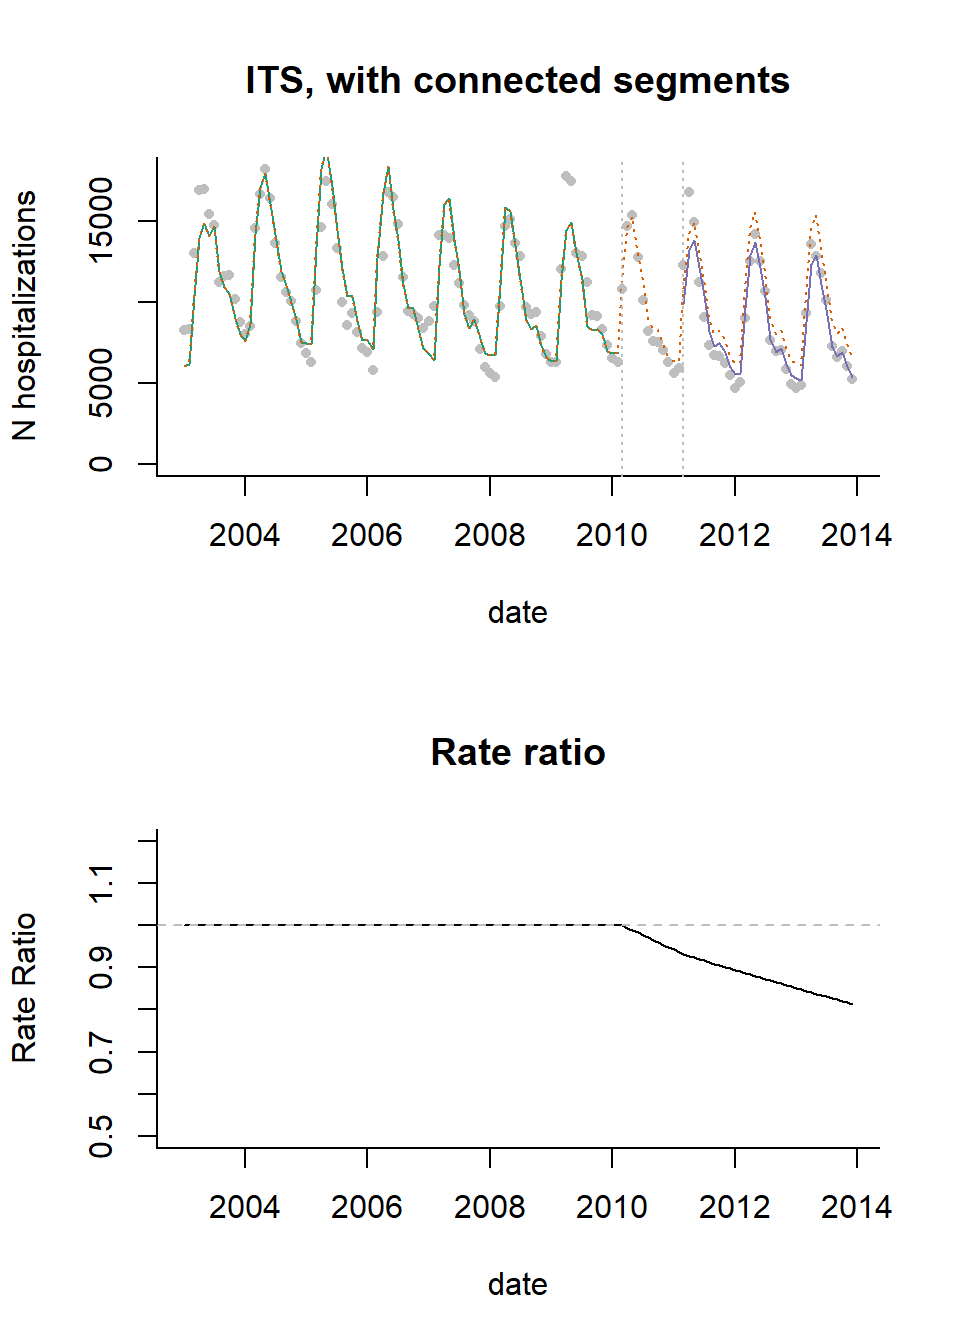
\includegraphics{WHO-guidance-on-use-of-administrative-data_files/figure-latex/unnamed-chunk-6-1.pdf}

\paragraph{ITS with leveling of the
slope}\label{its-with-leveling-of-the-slope}

This could be further modified to allow the slope to level out after a
certain time period (in this example, the post-vaccine trend levels out
36 months after vaccine introduction)

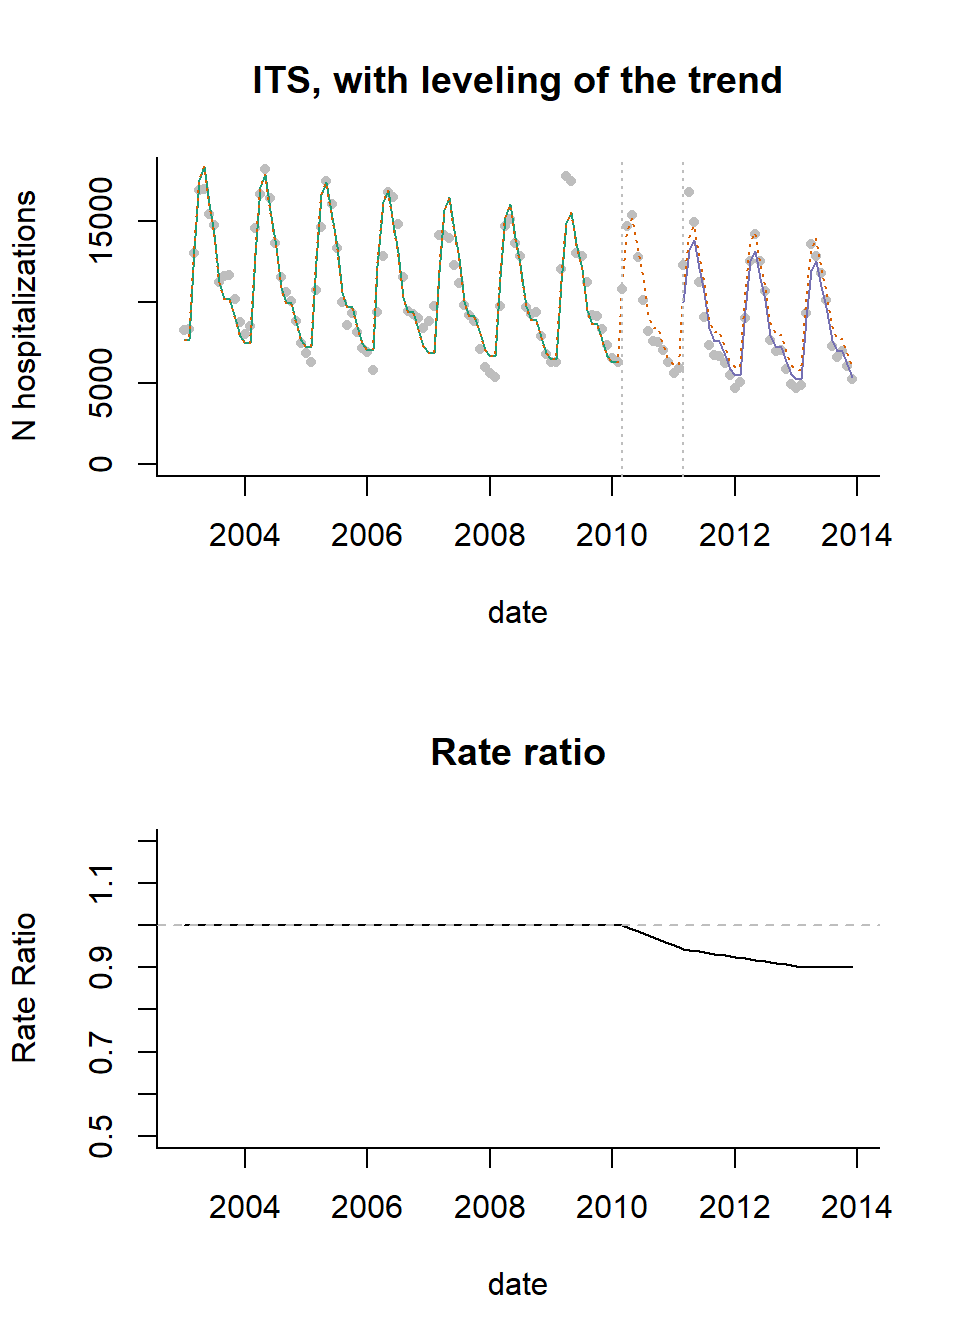
\includegraphics{WHO-guidance-on-use-of-administrative-data_files/figure-latex/unnamed-chunk-7-1.pdf}
\#\#\#

\textbf{Counterfactual} With an ITS model, the assumption is that the
trend from the pre-vaccine period would have continued with the same
slope into the post-vaccine period. To estimate the value of the
counterfactual at each time point, we use the regression model but hold
the terms representing post-vaccine changes in trend or level to 0 (no
change from the pre-vaccine trends and levels).

\textbf{Calculation of vaccine impact} Vaccine impact is measured in a
variety of ways with ITS models. Some authors report the actual change
in the slope parameter or change in the level. However, these values are
somewhat abstract and difficult to interpret from a public health
standpoint. It is more useful to calculate a relative change (rate
ratio) or an absolute change (rate difference) by comparing the fitted
value from the regression with the counterfactual value.

\textbf{Assumptions} A key assumption is that the linear trend in the
pre-vaccine period captures the important underlying trends and that
these trends would have continued at the same rate if the vaccine had
not been introduced. Assumptions also need to be made about which time
periods to include in the ramp-up period and whether the slope should
level out after a certain amount of time (and how much time should be
allowed). Some of these assumptions about the timing and shape of the
trajectory can be relaxed by using a flexible spline to capture
post-vaccine changes (For example, see van Deursen, \textbf{Vaccine},
2017)

\paragraph{The use of controls in ITS
analysis}\label{the-use-of-controls-in-its-analysis}

With this type of ITS analysis, there is a good chance that there are
changes in the time series that are not well-captured by the linear
trend assumption. There are 2 approaches that can be used to detect and
control for such patterns: control outcomes and control covariates

\textbf{Control Outcomes} With a control outcome, a different disease
that is not affected by the vaccine is chosen, and the same model that
was fit to the main outcome of interest is fit to this control time
series. If the

\textbf{Control covariates} It is also possible to include other time
series as control variables in the ITS regression model. The goal with
this approach is to adjust for time-varying confounders As an example,
if the outcome is pneumonia, and smoking rates are changing over time,
the rate of smoking in the population at each time point could be
included as a covariate. Alternatively,

*\textbf{Extensions}

-Change point models -Control covariates -Control outcomes -Holt-Winter,
ARIMA\ldots{}

\subsubsection{Synthetic controls}\label{synthetic-controls}

\textbf{Counterfactual} \textbf{Calculation of vaccine impact}
\textbf{Assumptions} *\textbf{Extensions}

\subsubsection{Other variations}\label{other-variations}

-incorporating controls into SC analyses -Dynamic transmission models

\textbf{How many years of data required?} -Requires pre-vaccine data

\textbf{What to do if you have an epidemic disease} All of these methods
assume that the disease patterns follow a preditable pattern and can be
captured either using a straight line relationship (ITS), or that the
relationship with control variables is stable. Therefore, these methods
are generally only appropriate for \textbf{endemic} diseases. For
diseases that are epidemic (e.g., meningococcal meningitis), other
approaches might be required that account for the dynamics of the
pathogen and the build-up of immunity in the population. If the epidemic
is widespread but the intervention is limited to a smaller region, it
might be possible to use the time series from an unvaccinated control
population as the control variable to generate a counterfactual in a
synthetic control-type analysis. Or it might be necessary to use a
dynamic transmission model that can capture non-linear dynamics (e.g., a
compartmental model with Susceptiple, Infected, and Resistant classes).

\subsection{Defining the study question and objectives
(CRISTIANA)}\label{defining-the-study-question-and-objectives-cristiana}

\subsection{Data Sources (international and national for both mortality
and hospitalization)
(Cristiana)}\label{data-sources-international-and-national-for-both-mortality-and-hospitalization-cristiana}

\subsection{Feasibility of conducting a time series analysis of
secondary data to assess vaccine impact (Concepts)
(CRISTIANA)}\label{feasibility-of-conducting-a-time-series-analysis-of-secondary-data-to-assess-vaccine-impact-concepts-cristiana}

\subsection{Data management (MOSTLY
CRISTIANA)}\label{data-management-mostly-cristiana}

\subsection{Data analysis (text + web based tutorial)
(DAN)}\label{data-analysis-text-web-based-tutorial-dan}

\subsubsection{Data formatting}\label{data-formatting}

To evaluate changes in disease rates associated with an intervention,
the first step is to format the data into a \textbf{time series}. Time
series enumerate the number of cases in a time period (e.g., week,
month, quarter, or year). We typically do this by starting with a
spreadsheet that has individual-level data, creating a variable that has
the date rounded rown to the date of the beginning of the nearest
week/month/quarter/year, and then adding up the number of cases that
occurred during that time period.

Ultimately we want to get a dataset that looks something like this, with
a column for the date, and a column for each of the diseases that we
want to enumerate

\begin{verbatim}
##          date pneumonia control1
## 1  2010-01-01        51      214
## 2  2010-02-01        51      215
## 3  2010-03-01        53      204
## 4  2010-04-01        50      234
## 5  2010-05-01        53      194
## 6  2010-06-01        64      193
## 7  2010-07-01        52      200
## 8  2010-08-01        57      209
## 9  2010-09-01        42      192
## 10 2010-10-01        43      212
## 11 2010-11-01        54      198
## 12 2010-12-01        42      197
## 13 2011-01-01        39      199
## 14 2011-02-01        50      198
## 15 2011-03-01        68      199
\end{verbatim}

If you have multiple strata, such as different age groups or regions,
the dataset will need to reflect this. In the table below, we have 3 age
groups, each with 5 observations. Each date/age group combination should
have only 1 row in this dataset.

\begin{verbatim}
##    age_group       date pneumonia control1
## 1          1 2010-01-01        54      185
## 2          1 2010-02-01        39      207
## 3          1 2010-03-01        54      176
## 4          1 2010-04-01        59      187
## 5          1 2010-05-01        68      202
## 6          2 2010-01-01        62      206
## 7          2 2010-02-01        51      218
## 8          2 2010-03-01        43      192
## 9          2 2010-04-01        52      182
## 10         2 2010-05-01        48      177
## 11         3 2010-01-01        43      186
## 12         3 2010-02-01        54      232
## 13         3 2010-03-01        57      214
## 14         3 2010-04-01        50      220
## 15         3 2010-05-01        57      181
\end{verbatim}

In the \emph{exercise}, we will learn how to take a individual-level
dataset that has 1 observation for each hospitalization/death and
convert it to a time series dataset.

\begin{itemize}
\tightlist
\item
  Descriptive analysis
\item
  Time series models
\item
  Synthetic Control analysis
\item
  Incorporating co-variates into the analyses
\item
  Exercises \#\#\#\# Converting individual-level data to time series
\end{itemize}

\subsection{Interpreting results (DAN)}\label{interpreting-results-dan}

 `dummy' results that highlight different scenarios (ie wide Cis with a
point estimate \textless{}\textless{}1, wide Cis with a point estimate
near 1, tight Cis with a point estimate near 1, tight Cis with a point
estimate far from 1) o Communicating and Presenting results effectively
(including suggested templates) (DAN AND CRIS)


\end{document}
